\documentclass[border=12pt]{standalone}
\usepackage{amsmath}
\usepackage{tikz}
\usetikzlibrary{arrows.meta,positioning}
\begin{document}
\begin{tabular}{c@{\hskip 1.4cm}c@{\hskip 1.4cm}c}
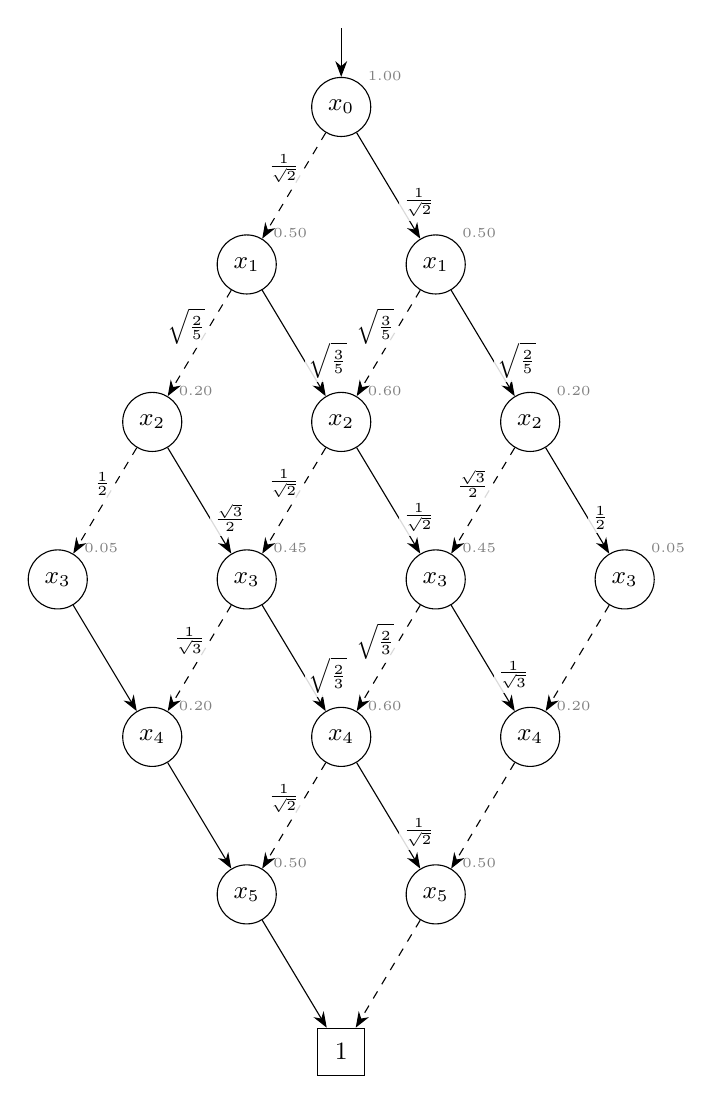
\begin{tikzpicture}[
    every node/.style={font=\small},
    nd/.style={circle, draw, minimum size=7.5mm, inner sep=0pt},
    tm/.style={rectangle, draw, minimum size=6mm, inner sep=2pt},
    e/.style={-{Stealth[length=2mm]}},
    lbl/.style={font=\scriptsize, inner sep=1.5pt, fill=white,
                fill opacity=0.85, text opacity=1},
    idl/.style={font=\tiny, inner sep=1pt, gray},
  ]
  \node[nd] (n15) at (0.00, 0.00) {$x_{0}$};
  \node[idl, above right=1pt of n15] {1.00};
  \node[nd] (n11) at (-1.20, -2.00) {$x_{1}$};
  \node[idl, above right=1pt of n11] {0.50};
  \node[nd] (n14) at (1.20, -2.00) {$x_{1}$};
  \node[idl, above right=1pt of n14] {0.50};
  \node[nd] (n7) at (-2.40, -4.00) {$x_{2}$};
  \node[idl, above right=1pt of n7] {0.20};
  \node[nd] (n10) at (0.00, -4.00) {$x_{2}$};
  \node[idl, above right=1pt of n10] {0.60};
  \node[nd] (n13) at (2.40, -4.00) {$x_{2}$};
  \node[idl, above right=1pt of n13] {0.20};
  \node[nd] (n3) at (-3.60, -6.00) {$x_{3}$};
  \node[idl, above right=1pt of n3] {0.05};
  \node[nd] (n6) at (-1.20, -6.00) {$x_{3}$};
  \node[idl, above right=1pt of n6] {0.45};
  \node[nd] (n9) at (1.20, -6.00) {$x_{3}$};
  \node[idl, above right=1pt of n9] {0.45};
  \node[nd] (n12) at (3.60, -6.00) {$x_{3}$};
  \node[idl, above right=1pt of n12] {0.05};
  \node[nd] (n2) at (-2.40, -8.00) {$x_{4}$};
  \node[idl, above right=1pt of n2] {0.20};
  \node[nd] (n5) at (0.00, -8.00) {$x_{4}$};
  \node[idl, above right=1pt of n5] {0.60};
  \node[nd] (n8) at (2.40, -8.00) {$x_{4}$};
  \node[idl, above right=1pt of n8] {0.20};
  \node[nd] (n1) at (-1.20, -10.00) {$x_{5}$};
  \node[idl, above right=1pt of n1] {0.50};
  \node[nd] (n4) at (1.20, -10.00) {$x_{5}$};
  \node[idl, above right=1pt of n4] {0.50};
  \node[tm] (term) at (0, -12.00) {$1$};
  \coordinate (in) at (0.00, 1.00);
  \draw[e] (in) -- (n15);
  \draw[e, solid] (n1) -- (term);
  \draw[e, solid] (n2) -- (n1);
  \draw[e, solid] (n3) -- (n2);
  \draw[e, dashed] (n4) -- (term);
  \draw[e, dashed] (n5) -- node[lbl, left, pos=0.34] {$\tfrac{1}{\sqrt{2}}$} (n1);
  \draw[e, solid] (n5) -- node[lbl, right, pos=0.66] {$\tfrac{1}{\sqrt{2}}$} (n4);
  \draw[e, dashed] (n6) -- node[lbl, left, pos=0.34] {$\tfrac{1}{\sqrt{3}}$} (n2);
  \draw[e, solid] (n6) -- node[lbl, right, pos=0.66] {$\sqrt{\tfrac{2}{3}}$} (n5);
  \draw[e, dashed] (n7) -- node[lbl, left, pos=0.34] {$\tfrac{1}{2}$} (n3);
  \draw[e, solid] (n7) -- node[lbl, right, pos=0.66] {$\tfrac{\sqrt{3}}{2}$} (n6);
  \draw[e, dashed] (n8) -- (n4);
  \draw[e, dashed] (n9) -- node[lbl, left, pos=0.34] {$\sqrt{\tfrac{2}{3}}$} (n5);
  \draw[e, solid] (n9) -- node[lbl, right, pos=0.66] {$\tfrac{1}{\sqrt{3}}$} (n8);
  \draw[e, dashed] (n10) -- node[lbl, left, pos=0.34] {$\tfrac{1}{\sqrt{2}}$} (n6);
  \draw[e, solid] (n10) -- node[lbl, right, pos=0.66] {$\tfrac{1}{\sqrt{2}}$} (n9);
  \draw[e, dashed] (n11) -- node[lbl, left, pos=0.34] {$\sqrt{\tfrac{2}{5}}$} (n7);
  \draw[e, solid] (n11) -- node[lbl, right, pos=0.66] {$\sqrt{\tfrac{3}{5}}$} (n10);
  \draw[e, dashed] (n12) -- (n8);
  \draw[e, dashed] (n13) -- node[lbl, left, pos=0.34] {$\tfrac{\sqrt{3}}{2}$} (n9);
  \draw[e, solid] (n13) -- node[lbl, right, pos=0.66] {$\tfrac{1}{2}$} (n12);
  \draw[e, dashed] (n14) -- node[lbl, left, pos=0.34] {$\sqrt{\tfrac{3}{5}}$} (n10);
  \draw[e, solid] (n14) -- node[lbl, right, pos=0.66] {$\sqrt{\tfrac{2}{5}}$} (n13);
  \draw[e, dashed] (n15) -- node[lbl, left, pos=0.34] {$\tfrac{1}{\sqrt{2}}$} (n11);
  \draw[e, solid] (n15) -- node[lbl, right, pos=0.66] {$\tfrac{1}{\sqrt{2}}$} (n14);
\end{tikzpicture}
&
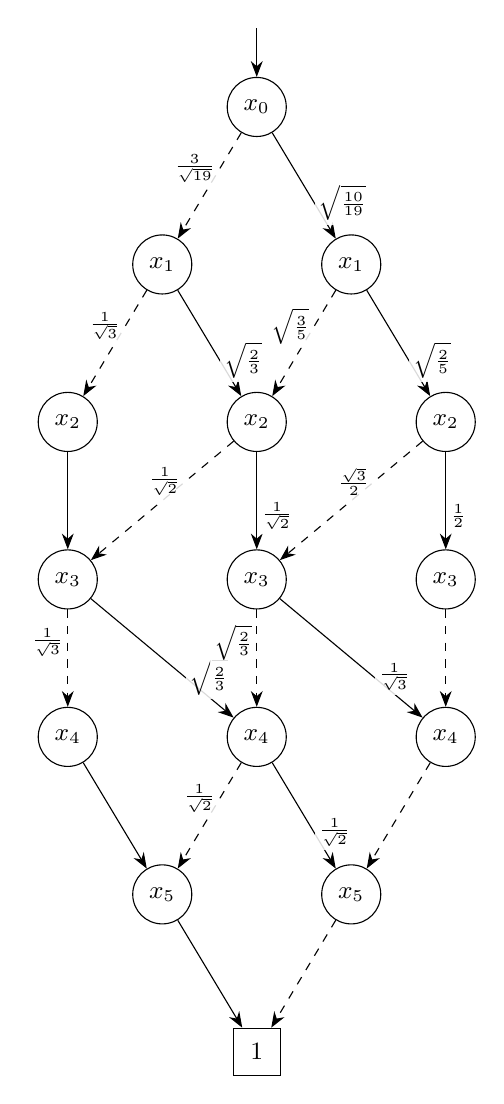
\begin{tikzpicture}[
    every node/.style={font=\small},
    nd/.style={circle, draw, minimum size=7.5mm, inner sep=0pt},
    tm/.style={rectangle, draw, minimum size=6mm, inner sep=2pt},
    e/.style={-{Stealth[length=2mm]}},
    lbl/.style={font=\scriptsize, inner sep=1.5pt, fill=white,
                fill opacity=0.85, text opacity=1},
    idl/.style={font=\tiny, inner sep=1pt, gray},
  ]
  \node[nd] (n18) at (0.00, 0.00) {$x_{0}$};
  \node[nd] (n17) at (-1.20, -2.00) {$x_{1}$};
  \node[nd] (n14) at (1.20, -2.00) {$x_{1}$};
  \node[nd] (n16) at (-2.40, -4.00) {$x_{2}$};
  \node[nd] (n10) at (0.00, -4.00) {$x_{2}$};
  \node[nd] (n13) at (2.40, -4.00) {$x_{2}$};
  \node[nd] (n6) at (-2.40, -6.00) {$x_{3}$};
  \node[nd] (n9) at (0.00, -6.00) {$x_{3}$};
  \node[nd] (n12) at (2.40, -6.00) {$x_{3}$};
  \node[nd] (n2) at (-2.40, -8.00) {$x_{4}$};
  \node[nd] (n5) at (0.00, -8.00) {$x_{4}$};
  \node[nd] (n8) at (2.40, -8.00) {$x_{4}$};
  \node[nd] (n1) at (-1.20, -10.00) {$x_{5}$};
  \node[nd] (n4) at (1.20, -10.00) {$x_{5}$};
  \node[tm] (term) at (0, -12.00) {$1$};
  \coordinate (in) at (0.00, 1.00);
  \draw[e] (in) -- (n18);
  \draw[e, solid] (n1) -- (term);
  \draw[e, solid] (n2) -- (n1);
  \draw[e, dashed] (n4) -- (term);
  \draw[e, dashed] (n5) -- node[lbl, left, pos=0.34] {$\tfrac{1}{\sqrt{2}}$} (n1);
  \draw[e, solid] (n5) -- node[lbl, right, pos=0.66] {$\tfrac{1}{\sqrt{2}}$} (n4);
  \draw[e, dashed] (n6) -- node[lbl, left, pos=0.34] {$\tfrac{1}{\sqrt{3}}$} (n2);
  \draw[e, solid] (n6) -- node[lbl, right, pos=0.66] {$\sqrt{\tfrac{2}{3}}$} (n5);
  \draw[e, dashed] (n8) -- (n4);
  \draw[e, dashed] (n9) -- node[lbl, left, pos=0.34] {$\sqrt{\tfrac{2}{3}}$} (n5);
  \draw[e, solid] (n9) -- node[lbl, right, pos=0.66] {$\tfrac{1}{\sqrt{3}}$} (n8);
  \draw[e, dashed] (n10) -- node[lbl, left, pos=0.34] {$\tfrac{1}{\sqrt{2}}$} (n6);
  \draw[e, solid] (n10) -- node[lbl, right, pos=0.66] {$\tfrac{1}{\sqrt{2}}$} (n9);
  \draw[e, dashed] (n12) -- (n8);
  \draw[e, dashed] (n13) -- node[lbl, left, pos=0.34] {$\tfrac{\sqrt{3}}{2}$} (n9);
  \draw[e, solid] (n13) -- node[lbl, right, pos=0.66] {$\tfrac{1}{2}$} (n12);
  \draw[e, dashed] (n14) -- node[lbl, left, pos=0.34] {$\sqrt{\tfrac{3}{5}}$} (n10);
  \draw[e, solid] (n14) -- node[lbl, right, pos=0.66] {$\sqrt{\tfrac{2}{5}}$} (n13);
  \draw[e, solid] (n16) -- (n6);
  \draw[e, dashed] (n17) -- node[lbl, left, pos=0.34] {$\tfrac{1}{\sqrt{3}}$} (n16);
  \draw[e, solid] (n17) -- node[lbl, right, pos=0.66] {$\sqrt{\tfrac{2}{3}}$} (n10);
  \draw[e, dashed] (n18) -- node[lbl, left, pos=0.34] {$\tfrac{3}{\sqrt{19}}$} (n17);
  \draw[e, solid] (n18) -- node[lbl, right, pos=0.66] {$\sqrt{\tfrac{10}{19}}$} (n14);
\end{tikzpicture}
&
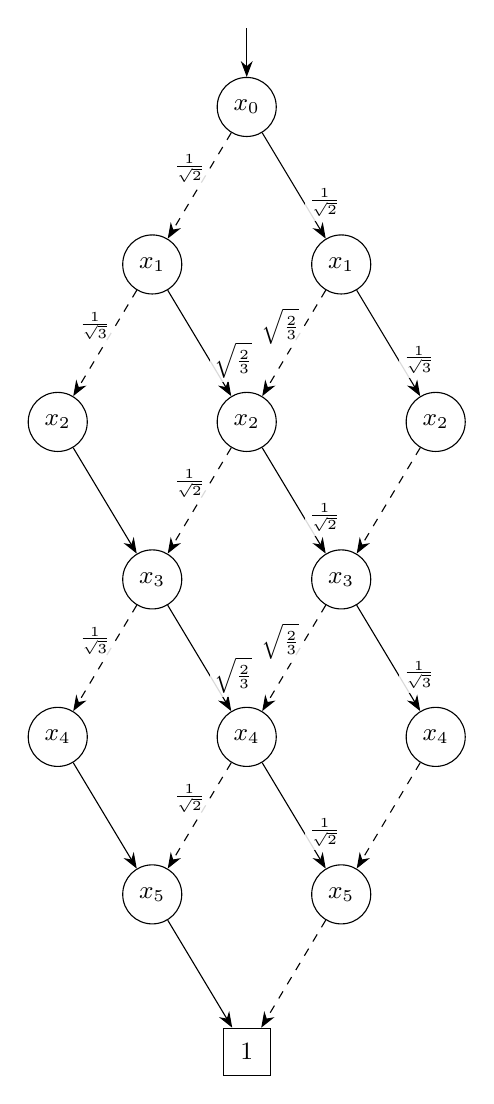
\begin{tikzpicture}[
    every node/.style={font=\small},
    nd/.style={circle, draw, minimum size=7.5mm, inner sep=0pt},
    tm/.style={rectangle, draw, minimum size=6mm, inner sep=2pt},
    e/.style={-{Stealth[length=2mm]}},
    lbl/.style={font=\scriptsize, inner sep=1.5pt, fill=white,
                fill opacity=0.85, text opacity=1},
    idl/.style={font=\tiny, inner sep=1pt, gray},
  ]
  \node[nd] (n21) at (0.00, 0.00) {$x_{0}$};
  \node[nd] (n17) at (-1.20, -2.00) {$x_{1}$};
  \node[nd] (n20) at (1.20, -2.00) {$x_{1}$};
  \node[nd] (n16) at (-2.40, -4.00) {$x_{2}$};
  \node[nd] (n10) at (0.00, -4.00) {$x_{2}$};
  \node[nd] (n19) at (2.40, -4.00) {$x_{2}$};
  \node[nd] (n6) at (-1.20, -6.00) {$x_{3}$};
  \node[nd] (n9) at (1.20, -6.00) {$x_{3}$};
  \node[nd] (n2) at (-2.40, -8.00) {$x_{4}$};
  \node[nd] (n5) at (0.00, -8.00) {$x_{4}$};
  \node[nd] (n8) at (2.40, -8.00) {$x_{4}$};
  \node[nd] (n1) at (-1.20, -10.00) {$x_{5}$};
  \node[nd] (n4) at (1.20, -10.00) {$x_{5}$};
  \node[tm] (term) at (0, -12.00) {$1$};
  \coordinate (in) at (0.00, 1.00);
  \draw[e] (in) -- (n21);
  \draw[e, solid] (n1) -- (term);
  \draw[e, solid] (n2) -- (n1);
  \draw[e, dashed] (n4) -- (term);
  \draw[e, dashed] (n5) -- node[lbl, left, pos=0.34] {$\tfrac{1}{\sqrt{2}}$} (n1);
  \draw[e, solid] (n5) -- node[lbl, right, pos=0.66] {$\tfrac{1}{\sqrt{2}}$} (n4);
  \draw[e, dashed] (n6) -- node[lbl, left, pos=0.34] {$\tfrac{1}{\sqrt{3}}$} (n2);
  \draw[e, solid] (n6) -- node[lbl, right, pos=0.66] {$\sqrt{\tfrac{2}{3}}$} (n5);
  \draw[e, dashed] (n8) -- (n4);
  \draw[e, dashed] (n9) -- node[lbl, left, pos=0.34] {$\sqrt{\tfrac{2}{3}}$} (n5);
  \draw[e, solid] (n9) -- node[lbl, right, pos=0.66] {$\tfrac{1}{\sqrt{3}}$} (n8);
  \draw[e, dashed] (n10) -- node[lbl, left, pos=0.34] {$\tfrac{1}{\sqrt{2}}$} (n6);
  \draw[e, solid] (n10) -- node[lbl, right, pos=0.66] {$\tfrac{1}{\sqrt{2}}$} (n9);
  \draw[e, solid] (n16) -- (n6);
  \draw[e, dashed] (n17) -- node[lbl, left, pos=0.34] {$\tfrac{1}{\sqrt{3}}$} (n16);
  \draw[e, solid] (n17) -- node[lbl, right, pos=0.66] {$\sqrt{\tfrac{2}{3}}$} (n10);
  \draw[e, dashed] (n19) -- (n9);
  \draw[e, dashed] (n20) -- node[lbl, left, pos=0.34] {$\sqrt{\tfrac{2}{3}}$} (n10);
  \draw[e, solid] (n20) -- node[lbl, right, pos=0.66] {$\tfrac{1}{\sqrt{3}}$} (n19);
  \draw[e, dashed] (n21) -- node[lbl, left, pos=0.34] {$\tfrac{1}{\sqrt{2}}$} (n17);
  \draw[e, solid] (n21) -- node[lbl, right, pos=0.66] {$\tfrac{1}{\sqrt{2}}$} (n20);
\end{tikzpicture}
\\[4pt] $D^{6}_{3}$ exact: 15 nodes & target $f=0.95$: 14 nodes, $F=0.95$ (level 3: $4 \to 3$) & target $f=0.9$: 13 nodes, $F=0.90$ (level 3: $4 \to 2$)
\\[10pt]
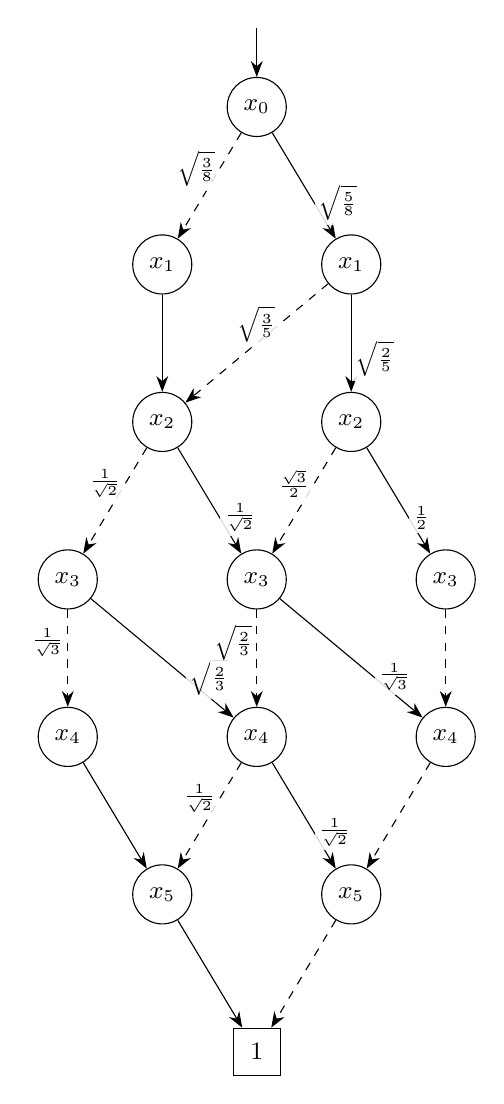
\begin{tikzpicture}[
    every node/.style={font=\small},
    nd/.style={circle, draw, minimum size=7.5mm, inner sep=0pt},
    tm/.style={rectangle, draw, minimum size=6mm, inner sep=2pt},
    e/.style={-{Stealth[length=2mm]}},
    lbl/.style={font=\scriptsize, inner sep=1.5pt, fill=white,
                fill opacity=0.85, text opacity=1},
    idl/.style={font=\tiny, inner sep=1pt, gray},
  ]
  \node[nd] (n23) at (0.00, 0.00) {$x_{0}$};
  \node[nd] (n22) at (-1.20, -2.00) {$x_{1}$};
  \node[nd] (n14) at (1.20, -2.00) {$x_{1}$};
  \node[nd] (n10) at (-1.20, -4.00) {$x_{2}$};
  \node[nd] (n13) at (1.20, -4.00) {$x_{2}$};
  \node[nd] (n6) at (-2.40, -6.00) {$x_{3}$};
  \node[nd] (n9) at (0.00, -6.00) {$x_{3}$};
  \node[nd] (n12) at (2.40, -6.00) {$x_{3}$};
  \node[nd] (n2) at (-2.40, -8.00) {$x_{4}$};
  \node[nd] (n5) at (0.00, -8.00) {$x_{4}$};
  \node[nd] (n8) at (2.40, -8.00) {$x_{4}$};
  \node[nd] (n1) at (-1.20, -10.00) {$x_{5}$};
  \node[nd] (n4) at (1.20, -10.00) {$x_{5}$};
  \node[tm] (term) at (0, -12.00) {$1$};
  \coordinate (in) at (0.00, 1.00);
  \draw[e] (in) -- (n23);
  \draw[e, solid] (n1) -- (term);
  \draw[e, solid] (n2) -- (n1);
  \draw[e, dashed] (n4) -- (term);
  \draw[e, dashed] (n5) -- node[lbl, left, pos=0.34] {$\tfrac{1}{\sqrt{2}}$} (n1);
  \draw[e, solid] (n5) -- node[lbl, right, pos=0.66] {$\tfrac{1}{\sqrt{2}}$} (n4);
  \draw[e, dashed] (n6) -- node[lbl, left, pos=0.34] {$\tfrac{1}{\sqrt{3}}$} (n2);
  \draw[e, solid] (n6) -- node[lbl, right, pos=0.66] {$\sqrt{\tfrac{2}{3}}$} (n5);
  \draw[e, dashed] (n8) -- (n4);
  \draw[e, dashed] (n9) -- node[lbl, left, pos=0.34] {$\sqrt{\tfrac{2}{3}}$} (n5);
  \draw[e, solid] (n9) -- node[lbl, right, pos=0.66] {$\tfrac{1}{\sqrt{3}}$} (n8);
  \draw[e, dashed] (n10) -- node[lbl, left, pos=0.34] {$\tfrac{1}{\sqrt{2}}$} (n6);
  \draw[e, solid] (n10) -- node[lbl, right, pos=0.66] {$\tfrac{1}{\sqrt{2}}$} (n9);
  \draw[e, dashed] (n12) -- (n8);
  \draw[e, dashed] (n13) -- node[lbl, left, pos=0.34] {$\tfrac{\sqrt{3}}{2}$} (n9);
  \draw[e, solid] (n13) -- node[lbl, right, pos=0.66] {$\tfrac{1}{2}$} (n12);
  \draw[e, dashed] (n14) -- node[lbl, left, pos=0.34] {$\sqrt{\tfrac{3}{5}}$} (n10);
  \draw[e, solid] (n14) -- node[lbl, right, pos=0.66] {$\sqrt{\tfrac{2}{5}}$} (n13);
  \draw[e, solid] (n22) -- (n10);
  \draw[e, dashed] (n23) -- node[lbl, left, pos=0.34] {$\sqrt{\tfrac{3}{8}}$} (n22);
  \draw[e, solid] (n23) -- node[lbl, right, pos=0.66] {$\sqrt{\tfrac{5}{8}}$} (n14);
\end{tikzpicture}
&
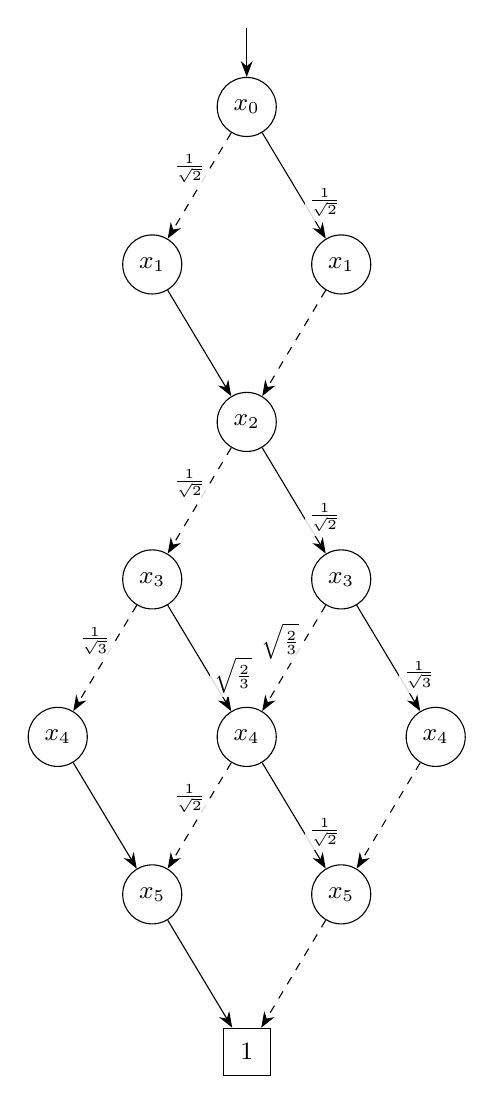
\begin{tikzpicture}[
    every node/.style={font=\small},
    nd/.style={circle, draw, minimum size=7.5mm, inner sep=0pt},
    tm/.style={rectangle, draw, minimum size=6mm, inner sep=2pt},
    e/.style={-{Stealth[length=2mm]}},
    lbl/.style={font=\scriptsize, inner sep=1.5pt, fill=white,
                fill opacity=0.85, text opacity=1},
    idl/.style={font=\tiny, inner sep=1pt, gray},
  ]
  \node[nd] (n31) at (0.00, 0.00) {$x_{0}$};
  \node[nd] (n22) at (-1.20, -2.00) {$x_{1}$};
  \node[nd] (n30) at (1.20, -2.00) {$x_{1}$};
  \node[nd] (n10) at (0.00, -4.00) {$x_{2}$};
  \node[nd] (n6) at (-1.20, -6.00) {$x_{3}$};
  \node[nd] (n9) at (1.20, -6.00) {$x_{3}$};
  \node[nd] (n2) at (-2.40, -8.00) {$x_{4}$};
  \node[nd] (n5) at (0.00, -8.00) {$x_{4}$};
  \node[nd] (n8) at (2.40, -8.00) {$x_{4}$};
  \node[nd] (n1) at (-1.20, -10.00) {$x_{5}$};
  \node[nd] (n4) at (1.20, -10.00) {$x_{5}$};
  \node[tm] (term) at (0, -12.00) {$1$};
  \coordinate (in) at (0.00, 1.00);
  \draw[e] (in) -- (n31);
  \draw[e, solid] (n1) -- (term);
  \draw[e, solid] (n2) -- (n1);
  \draw[e, dashed] (n4) -- (term);
  \draw[e, dashed] (n5) -- node[lbl, left, pos=0.34] {$\tfrac{1}{\sqrt{2}}$} (n1);
  \draw[e, solid] (n5) -- node[lbl, right, pos=0.66] {$\tfrac{1}{\sqrt{2}}$} (n4);
  \draw[e, dashed] (n6) -- node[lbl, left, pos=0.34] {$\tfrac{1}{\sqrt{3}}$} (n2);
  \draw[e, solid] (n6) -- node[lbl, right, pos=0.66] {$\sqrt{\tfrac{2}{3}}$} (n5);
  \draw[e, dashed] (n8) -- (n4);
  \draw[e, dashed] (n9) -- node[lbl, left, pos=0.34] {$\sqrt{\tfrac{2}{3}}$} (n5);
  \draw[e, solid] (n9) -- node[lbl, right, pos=0.66] {$\tfrac{1}{\sqrt{3}}$} (n8);
  \draw[e, dashed] (n10) -- node[lbl, left, pos=0.34] {$\tfrac{1}{\sqrt{2}}$} (n6);
  \draw[e, solid] (n10) -- node[lbl, right, pos=0.66] {$\tfrac{1}{\sqrt{2}}$} (n9);
  \draw[e, solid] (n22) -- (n10);
  \draw[e, dashed] (n30) -- (n10);
  \draw[e, dashed] (n31) -- node[lbl, left, pos=0.34] {$\tfrac{1}{\sqrt{2}}$} (n22);
  \draw[e, solid] (n31) -- node[lbl, right, pos=0.66] {$\tfrac{1}{\sqrt{2}}$} (n30);
\end{tikzpicture}
&
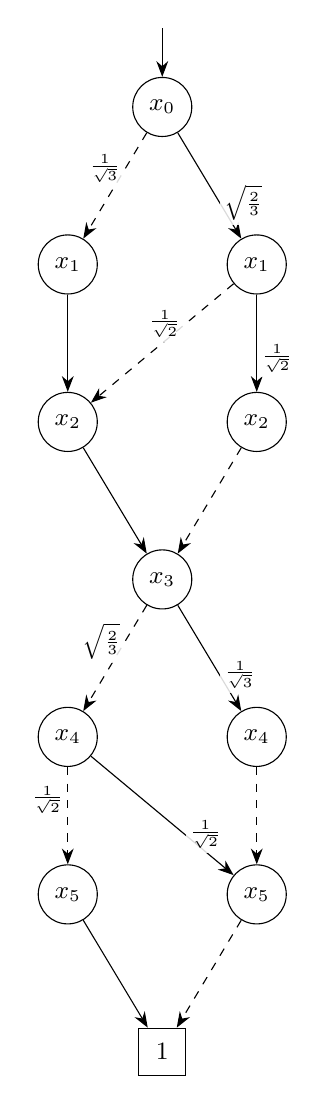
\begin{tikzpicture}[
    every node/.style={font=\small},
    nd/.style={circle, draw, minimum size=7.5mm, inner sep=0pt},
    tm/.style={rectangle, draw, minimum size=6mm, inner sep=2pt},
    e/.style={-{Stealth[length=2mm]}},
    lbl/.style={font=\scriptsize, inner sep=1.5pt, fill=white,
                fill opacity=0.85, text opacity=1},
    idl/.style={font=\tiny, inner sep=1pt, gray},
  ]
  \node[nd] (n51) at (0.00, 0.00) {$x_{0}$};
  \node[nd] (n49) at (-1.20, -2.00) {$x_{1}$};
  \node[nd] (n50) at (1.20, -2.00) {$x_{1}$};
  \node[nd] (n48) at (-1.20, -4.00) {$x_{2}$};
  \node[nd] (n19) at (1.20, -4.00) {$x_{2}$};
  \node[nd] (n9) at (0.00, -6.00) {$x_{3}$};
  \node[nd] (n5) at (-1.20, -8.00) {$x_{4}$};
  \node[nd] (n8) at (1.20, -8.00) {$x_{4}$};
  \node[nd] (n1) at (-1.20, -10.00) {$x_{5}$};
  \node[nd] (n4) at (1.20, -10.00) {$x_{5}$};
  \node[tm] (term) at (0, -12.00) {$1$};
  \coordinate (in) at (0.00, 1.00);
  \draw[e] (in) -- (n51);
  \draw[e, solid] (n1) -- (term);
  \draw[e, dashed] (n4) -- (term);
  \draw[e, dashed] (n5) -- node[lbl, left, pos=0.34] {$\tfrac{1}{\sqrt{2}}$} (n1);
  \draw[e, solid] (n5) -- node[lbl, right, pos=0.66] {$\tfrac{1}{\sqrt{2}}$} (n4);
  \draw[e, dashed] (n8) -- (n4);
  \draw[e, dashed] (n9) -- node[lbl, left, pos=0.34] {$\sqrt{\tfrac{2}{3}}$} (n5);
  \draw[e, solid] (n9) -- node[lbl, right, pos=0.66] {$\tfrac{1}{\sqrt{3}}$} (n8);
  \draw[e, dashed] (n19) -- (n9);
  \draw[e, solid] (n48) -- (n9);
  \draw[e, solid] (n49) -- (n48);
  \draw[e, dashed] (n50) -- node[lbl, left, pos=0.34] {$\tfrac{1}{\sqrt{2}}$} (n48);
  \draw[e, solid] (n50) -- node[lbl, right, pos=0.66] {$\tfrac{1}{\sqrt{2}}$} (n19);
  \draw[e, dashed] (n51) -- node[lbl, left, pos=0.34] {$\tfrac{1}{\sqrt{3}}$} (n49);
  \draw[e, solid] (n51) -- node[lbl, right, pos=0.66] {$\sqrt{\tfrac{2}{3}}$} (n50);
\end{tikzpicture}
\\[4pt] target $f=0.8$: 13 nodes, $F=0.80$ (level 2: $3 \to 2$, level 3: $4 \to 3$) & target $f=0.6$: 11 nodes, $F=0.60$ (level 2: $3 \to 1$, level 3: $4 \to 2$) & target $f=0.3$: 10 nodes, $F=0.45$ (level 2: $3 \to 2$, level 3: $4 \to 1$, level 4: $3 \to 2$)
\end{tabular}
\end{document}